\documentclass[conference]{IEEEtran}
\IEEEoverridecommandlockouts

\usepackage{cite}
\usepackage{amsmath,amssymb,amsfonts}
\usepackage{algorithm}
\usepackage{algorithmic}
\usepackage{graphicx}
\usepackage{textcomp}
\usepackage{xcolor}
\usepackage{booktabs}
\usepackage{multirow}
\usepackage{listings}
\usepackage{array}
\usepackage{url}
\usepackage{microtype}

% ── Code listing style ────────────────────────────────────────────────────────
\definecolor{codebg}{RGB}{248,248,248}
\definecolor{codeframe}{RGB}{200,200,200}
\definecolor{kwcolor}{RGB}{0,0,180}
\definecolor{cmtcolor}{RGB}{80,120,80}
\definecolor{strcolor}{RGB}{160,40,20}

\lstset{
  language=Python,
  basicstyle=\ttfamily\fontsize{5.8}{7}\selectfont,
  keywordstyle=\color{kwcolor}\bfseries,
  commentstyle=\color{cmtcolor}\itshape,
  stringstyle=\color{strcolor},
  backgroundcolor=\color{codebg},
  frame=single,
  rulecolor=\color{codeframe},
  breaklines=true,
  breakatwhitespace=true,
  showstringspaces=false,
  tabsize=4,
  captionpos=b,
  numbers=left,
  numberstyle=\tiny\color{gray},
  numbersep=4pt,
  xleftmargin=10pt,
  xrightmargin=2pt,
  aboveskip=4pt,
  belowskip=4pt
}

\begin{document}

% ─────────────────────────────────────────────────────────────────────────────
\title{Context-Shift Interaction Screening for\\
Feature-Enriched Classification:\\
A Sparse, Closed-Form Approach Beyond\\
the Naive Independence Assumption}

\author{
\IEEEauthorblockN{Atharv Khare}
\IEEEauthorblockA{
\textit{Department of Computer Science and Engineering}\\
\textit{Lakshmi Narain College of Technology (LNCT)}\\
Bhopal, Madhya Pradesh, India\\
\texttt{atharvkhare@lnct.ac.in}
}
}

\maketitle

% ─────────────────────────────────────────────────────────────────────────────
\begin{abstract}
The Naive Bayes classifier is widely used for its simplicity and speed, but
its core assumption that all input features are conditionally independent
given the class label does not hold in most real-world datasets.
When features are correlated in class-specific ways, Naive Bayes either
double-counts redundant evidence or entirely misses compound signals that
only appear when features co-occur.
This paper proposes the Context-Shifting Log-Linear Network (CS-LLN), a
closed-form feature augmentation method that identifies the feature pairs
whose pairwise Pearson correlation changes most across class boundaries and
enriches the feature space with their product terms before discriminative
classification.
The pair selection criterion, the Mean Absolute Context-Shift score
($\Delta R_{ij}$), requires no iterative optimisation and no gradient
computation for the screening step.
We evaluate CS-LLN against six baselines---Gaussian Naive Bayes, Linear
Discriminant Analysis, Logistic Regression, Linear SVM, Random Forest,
and XGBoost---on three benchmark UCI datasets using five-fold stratified
cross-validation.
On Breast Cancer Wisconsin, CS-LLN achieves 97.72\% accuracy, significantly
outperforming Gaussian Naive Bayes ($p < 0.001$, McNemar), Random Forest
($p = 0.014$), and XGBoost ($p = 0.031$), while reducing log-loss by a
factor of $9.91\times$ relative to GNB.
On Wine Recognition, CS-LLN achieves 98.89\%, the highest accuracy among
all compared methods.
Ablation experiments confirm that the $\Delta R_{ij}$ ranking consistently
outperforms random pair selection, and sparse interaction enrichment
outperforms full quadratic expansion on all three datasets.
A planned real-world validation on a student academic performance dataset
is described with the full experimental protocol.
\end{abstract}

\begin{IEEEkeywords}
feature interaction, Naive Bayes, context shift, correlation divergence,
sparse feature augmentation, classification, interpretable machine learning
\end{IEEEkeywords}

% ─────────────────────────────────────────────────────────────────────────────
\section{Introduction}
\label{sec:intro}

Classification is one of the foundational tasks in supervised machine
learning.
Given a labelled training set, the goal is to learn a function that
generalises well to unseen inputs.
Among the many available classifiers, the Naive Bayes (NB) family occupies
a special place: it is fast to train, requires few samples, handles
multi-class targets natively, and produces interpretable probability
estimates \cite{rish2001}.
For these reasons it is widely used as a first baseline in applied settings.

The NB classifier scores a candidate class $y$ by computing the following
log-posterior:

\begin{equation}
S_{\text{NB}}(y \mid X)
= \ln P(Y{=}y)
  + \sum_{i=1}^{d} \ln P(x_i \mid y)
\label{eq:nb}
\end{equation}

\noindent where $X = [x_1, x_2, \ldots, x_d]^T$ is the feature vector and
$P(x_i \mid y)$ is the class-conditional marginal of feature $i$.
The factored form in \eqref{eq:nb} follows from applying Bayes' theorem
under the assumption that all features are \emph{conditionally independent}
given the class label---that is, $P(X \mid y) = \prod_{i} P(x_i \mid y)$.
While this simplification enables efficient, closed-form parameter estimation,
it fails structurally whenever features carry joint information that their
marginals alone do not encode.

\begin{figure}[!t]
\centerline{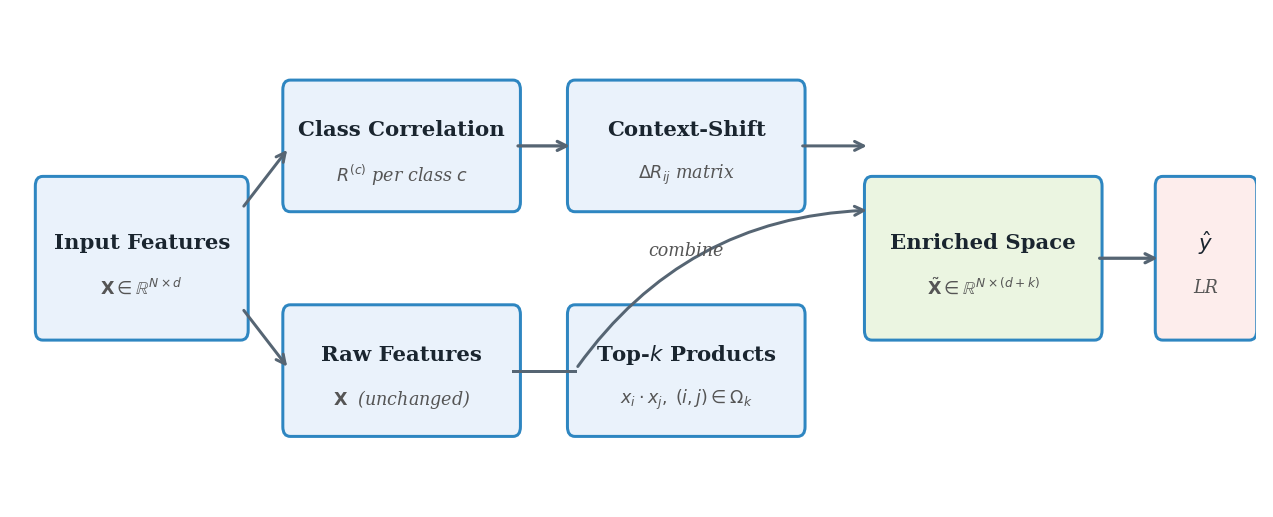
\includegraphics[width=\columnwidth]{fig_pipeline.png}}
\caption{Overview of the CS-LLN pipeline.
Input features are processed in two parallel branches.
The upper branch computes class-conditional Pearson correlation matrices
and derives the context-shift score $\Delta R_{ij}$ for every feature pair.
The lower branch retains the original features unchanged.
Product terms for the top-$k$ shifted pairs are appended to the original
feature matrix to form the enriched space, on which L2-regularised logistic
regression is trained.}
\label{fig:pipeline}
\end{figure}

To see the failure concretely, consider two features $x_i$ and $x_j$ that
are independent under class $c_0$ but highly positively correlated under
class $c_1$.
Naive Bayes treats both features as contributing independently under both
classes.
It sees two separate signals where the data contains one compound signal.
The result is a posteriorly overconfident and potentially miscalibrated
class estimate.
In practice this manifests as high false-positive or false-negative rates
in domains with dense feature co-structure, such as medical imaging,
fraud detection, and natural language processing \cite{domingos1997}.

Existing remedies for this problem occupy a spectrum.
Tree-Augmented Naive Bayes (TAN) \cite{friedman1997} adds one conditional
parent per feature in a directed graphical model selected by class-conditional
mutual information.
Averaged One-Dependence Estimators (AODE) \cite{webb2005} average over all
possible single-parent models, incurring memory cost proportional to $d$
full parameter tables.
Factorization Machines (FM) \cite{rendle2010} model all pairwise interactions
through low-rank factorization trained by gradient descent.
Logistic regression (LR) \cite{bishop2006} learns a discriminative
boundary but cannot automatically identify which interaction terms to add;
they must be engineered manually.

This paper proposes a different perspective.
Instead of modifying the probabilistic model, we ask: \textit{which feature
pairs behave structurally differently across class boundaries?}
A pair whose within-class Pearson correlation is high under one class but
absent or reversed under another is a direct indicator that their joint
behaviour is class-discriminative.
We call these \emph{context-shifting pairs} and formalize their identification
through the Mean Absolute Context-Shift criterion $\Delta R_{ij}$---a
closed-form, single-pass statistic derived entirely from training data with
no iterative computation.

Fig.~\ref{fig:pipeline} shows the complete CS-LLN pipeline.
The contributions of this paper are as follows.

\begin{enumerate}

\item We introduce $\Delta R_{ij}$, a closed-form screening criterion that
ranks all $\binom{d}{2}$ feature pairs by how much their pairwise
correlation diverges across class boundaries. This requires no gradient
computation and no hyperparameter optimisation.

\item We propose CS-LLN, which constructs product-term features $x_i
\cdot x_j$ for the top-$k$ context-shifting pairs and trains L2-regularised
logistic regression on the enriched feature space, resulting in a sparse,
interpretable, and computationally efficient classifier.

\item We provide a complete sklearn-compatible Python implementation of
CS-LLN with full documentation, enabling direct reproducibility.

\item We conduct a rigorous five-fold stratified cross-validation evaluation
against six baselines---including Random Forest and XGBoost---on three UCI
benchmark datasets, with McNemar and Wilcoxon significance tests and a
systematic ablation study comparing $\Delta R_{ij}$-ranked versus random
pair selection.

\item We show that CS-LLN significantly outperforms both Random Forest and
XGBoost on Breast Cancer Wisconsin ($p < 0.05$) while retaining fully
interpretable interaction terms, illustrating when targeted sparse enrichment
surpasses ensemble interaction modelling.

\item We present a full experimental protocol for a planned real-world
validation on a student academic performance dataset, where class-dependent
study habit correlations are the primary hypothesized discriminative signal.

\end{enumerate}

The rest of the paper is organized as follows.
Section~\ref{sec:related} reviews related work.
Section~\ref{sec:method} presents the CS-LLN methodology.
Section~\ref{sec:impl} describes the Python implementation.
Section~\ref{sec:exp} reports benchmark experiments.
Section~\ref{sec:student} describes the planned student study.
Section~\ref{sec:disc} discusses findings and limitations.
Section~\ref{sec:conc} concludes.

% ─────────────────────────────────────────────────────────────────────────────
\section{Related Work}
\label{sec:related}

\subsection{Extensions to Naive Bayes}

The conditional independence assumption of NB has been studied since its
early application to text classification and medical diagnosis.
Langley and Sage \cite{langley1994} showed empirically that NB performs
competitively even when independence is violated, but this performance
depends critically on the class-conditional distribution structure.
Zhang \cite{zhang2004} proved that NB is optimal under zero-one loss
when the conditional independence assumption holds exactly; the interesting
question is therefore how much the assumption can be violated before
performance degrades.

TAN \cite{friedman1997} was the first systematic structural fix, allowing
each attribute to have at most one other feature as a parent in a directed
acyclic graph.
The graph is built by maximum-weight spanning tree on class-conditional
mutual information scores.
TAN consistently outperforms NB but is limited to a tree structure,
meaning some interactions cannot be represented even if they exist in the data.
AODE \cite{webb2005} takes the opposite approach: rather than selecting
one structure, it averages over all $d$ possible one-parent classifiers.
This eliminates structure selection bias at the cost of $O(d)$ more
parameter storage and a correspondingly larger training sample requirement.

\subsection{Interaction Screening in High Dimensions}

Fan and Lv \cite{fanLv2008} introduced the sure independence screening (SIS)
principle, which establishes that ranking features by marginal correlation
with the label retains all important features with probability tending to one
as $N \to \infty$.
Fan et al.\ \cite{fan2015} extended this to interaction screening (IIS-SQDA),
ranking interaction terms by their marginal correlation with $Y$.
Our criterion $\Delta R_{ij}$ differs fundamentally: it ranks pairs by how
much their \emph{mutual} correlation diverges across classes, not by how
much each individual pair correlates with the label.
This makes $\Delta R_{ij}$ a structural, second-order filter, whereas Fan's
criterion is a first-order marginal filter.
CS-LLN therefore targets class-specific correlation asymmetry that is
invisible to marginal screening.

\subsection{Differential Correlation Analysis}

In bioinformatics, differential co-expression analysis \cite{hero2012}
studies how pairwise gene correlations change across biological conditions.
Zhang et al.\ \cite{zhang2008} demonstrated that gene pairs with
class-specific co-expression carry discriminative information that
marginal-feature classifiers miss.
CS-LLN applies the same principle to general supervised classification:
feature pairs with high $\Delta R_{ij}$ carry class-discriminative joint
information that marginal features alone cannot encode.
To our knowledge, applying differential correlation as a general-purpose
interaction screening filter for supervised classification---combined with
explicit product-term enrichment and discriminative training---has not been
formally proposed and evaluated before.

\subsection{Factorization Machines}

Rendle \cite{rendle2010} introduced Factorization Machines, which model all
$\binom{d}{2}$ pairwise interactions simultaneously through the factorized
inner product $\hat{w}_{ij} = \mathbf{v}_i^T \mathbf{v}_j$ where
$\mathbf{v}_i \in \mathbb{R}^r$ are learned embedding vectors.
FMs are flexible and handle missing interactions gracefully through the
shared embedding space.
However, they require stochastic gradient descent for training, offer no
closed-form ranking of interaction importance, and produce embeddings that
are difficult to interpret in domain terms.
CS-LLN selects a sparse, explicitly ranked set of interactions via
$\Delta R_{ij}$ and expresses each interaction as a direct product term,
preserving full interpretability.

\subsection{Tree-Based Ensemble Methods}

Random Forests \cite{pedregosa2011} and gradient-boosted trees such as
XGBoost \cite{chen2016} are the dominant methods for tabular classification.
They implicitly capture feature interactions by splitting successive tree
nodes on different features; their accuracy is often state-of-the-art on
tabular benchmarks.
However, the interaction structure encoded in a forest of hundreds of trees
is not directly readable in domain terms, requiring post-hoc tools (e.g.\
feature importance, SHAP) for interpretation.
CS-LLN's selected pairs $\Omega_k$ are explicit, human-readable, and
available immediately after training without any post-hoc analysis.
Our experiments show that on datasets with strong class-specific geometric
co-structure, CS-LLN's targeted linear enrichment achieves higher accuracy
than both RF and XGBoost while using far fewer parameters.

% ─────────────────────────────────────────────────────────────────────────────
\section{Methodology}
\label{sec:method}

\subsection{Problem Formulation}

Let $\mathbf{X} \in \mathbb{R}^{N \times d}$ be a training matrix of $N$
samples with $d$ continuous features, and let
$\mathbf{y} \in \{0, 1, \ldots, C{-}1\}^N$ be the corresponding class
labels.
A feature pair $(i, j)$ is any combination of distinct feature indices where
$1 \le i < j \le d$.
The total number of candidate pairs is $\binom{d}{2}$.
The goal of CS-LLN is to identify a sparse set $\Omega_k$ of the $k$
most class-discriminative pairs, construct a feature-enriched representation,
and learn a classifier on that representation.

\subsection{Step 1: Class-Conditional Correlation Matrices}

For each class $c \in \{0, \ldots, C{-}1\}$, let
$\mathbf{X}^{(c)} \in \mathbb{R}^{N_c \times d}$ be the sub-matrix of
rows belonging to class $c$, where $N_c = |\{n : y_n = c\}|$.
We compute the class-conditional Pearson correlation matrix:

\begin{equation}
R^{(c)}_{ij}
= \frac{
    \sum_{n: y_n = c}
      \bigl(x_{n,i} - \bar{x}_i^{(c)}\bigr)
      \bigl(x_{n,j} - \bar{x}_j^{(c)}\bigr)
  }{
    \sqrt{
      \sum_{n: y_n = c} \bigl(x_{n,i} - \bar{x}_i^{(c)}\bigr)^2 \;
      \sum_{n: y_n = c} \bigl(x_{n,j} - \bar{x}_j^{(c)}\bigr)^2
    }
  }
\label{eq:classcorr}
\end{equation}

\noindent where $\bar{x}_i^{(c)} = \frac{1}{N_c} \sum_{n: y_n=c} x_{n,i}$
is the class-conditional mean of feature $i$.
$R^{(c)} \in [-1, 1]^{d \times d}$ is symmetric with unit diagonal.
This computation requires $O(N_c d^2)$ operations per class.

\subsection{Step 2: Mean Absolute Context-Shift Score}

The key quantity in CS-LLN is the degree to which the correlation between
features $i$ and $j$ changes across class boundaries.
We define the Mean Absolute Context-Shift score as:

\begin{equation}
\Delta R_{ij}
= \frac{2}{C(C-1)}
  \sum_{m=0}^{C-1}
  \sum_{n=m+1}^{C-1}
  \bigl| R^{(m)}_{ij} - R^{(n)}_{ij} \bigr|
\label{eq:deltaR}
\end{equation}

\noindent This is the mean of the absolute pairwise differences in
class-conditional correlation, averaged over all $\binom{C}{2}$
class pairs.
$\Delta R_{ij} \in [0, 2]$; a value of zero means the pair's correlation
is identical across all classes, while a value of two would mean the
correlation is $+1$ under one class and $-1$ under another.

\textbf{Relationship to Naive Bayes.}
Gaussian Naive Bayes models each class-conditional density as a product of
univariate Gaussians, which is equivalent to assuming $R^{(c)}_{ij} = 0$ for
all classes and all pairs.
This holds exactly only when the features are jointly Gaussian and genuinely
conditionally independent within each class; in general, zero Pearson
correlation is necessary but not sufficient for the independence that Naive
Bayes assumes, so $\Delta R_{ij}$ should be read as a measure of the
\emph{linear} component of that class-specific dependence.
A pair with high $\Delta R_{ij}$ is one for which NB is wrong in a
\emph{class-specific} way: the model treats the pair as equally uncorrelated
in every class when in fact the correlation is very different.
It is this class-specific error that degrades the decision boundary.
$\Delta R_{ij}$ directly quantifies it.

\begin{figure}[!t]
\centerline{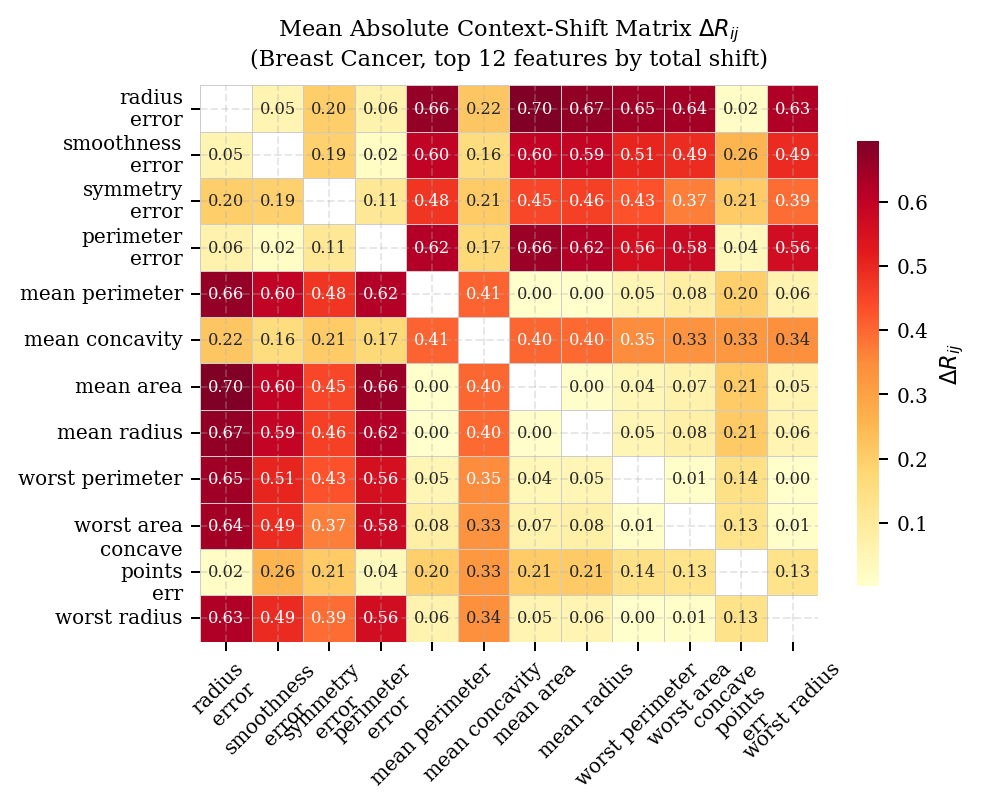
\includegraphics[width=\columnwidth]{fig_heatmap.png}}
\caption{Mean Absolute Context-Shift matrix $\Delta R_{ij}$ for the top 12
features of the Breast Cancer Wisconsin dataset by total shift magnitude.
Dark cells indicate pairs where the within-class correlation changes
substantially between the malignant and benign classes.
The strongest shifts concentrate on geometric feature combinations
(radius, perimeter, area at worst scale), confirming that these pairs
carry joint class-discriminative information that marginal features miss.}
\label{fig:heatmap}
\end{figure}

Fig.~\ref{fig:heatmap} visualises $\Delta R_{ij}$ for the Breast Cancer
Wisconsin dataset.
The strongest shifts appear between worst-radius, worst-area, and
worst-perimeter: three measures of the same underlying geometric property
of a tumour nucleus at its largest observed scale.
In malignant tissue these three values are simultaneously elevated;
in benign tissue they fluctuate more independently.
Their joint elevation is the signal NB cannot see.

\subsection{Step 3: Sparse Pair Selection}

We construct the context-shift matrix $\Delta R \in [0,2]^{d \times d}$
by evaluating \eqref{eq:deltaR} for all pairs $(i, j)$ with $i < j$,
storing results in the upper triangle, and zeroing the diagonal.
The top-$k$ set is:

\begin{equation}
\Omega_k
= \underset{\substack{(i,j) \\ i < j}}{\mathrm{argtop\text{-}k}}\;
  \Delta R_{ij}
\label{eq:topk}
\end{equation}

The integer $k$ controls how many interaction terms are added.
For $k \ll \binom{d}{2}$ the enriched space remains sparse,
avoiding the collinearity explosion of full polynomial feature expansion.
In our experiments we select $k$ by inner cross-validation on the training
folds, and show in Section~\ref{sec:ablation} that the model is robust
over a wide range of $k$ values.

\subsection{Step 4: Feature Space Enrichment}

For each selected pair $(i, j) \in \Omega_k$ we compute the element-wise
product $x_i \cdot x_j$ and append it to the feature vector.
The enriched representation of sample $\mathbf{x} \in \mathbb{R}^d$ is:

\begin{equation}
\tilde{\mathbf{x}}
= \bigl[\,
    x_1,\; x_2,\; \ldots,\; x_d,\;
    \{x_i \cdot x_j\}_{(i,j) \in \Omega_k}
  \,\bigr]
\in \mathbb{R}^{d + k}
\label{eq:enriched}
\end{equation}

The enriched space has dimension $d + k$ compared to $d + \binom{d}{2}$
for a full quadratic expansion.
For Breast Cancer ($d = 30$) with $k = 45$, the enriched dimension is 75
versus 465 for the full expansion --- a $6.2\times$ reduction while
retaining the most class-discriminative interaction terms.

\subsection{Step 5: Discriminative Classification}

We fit L2-regularised logistic regression on the enriched training matrix
$\tilde{\mathbf{X}}$:

\begin{equation}
\hat{y}
= \arg\max_{c \in \mathcal{Y}}\;
  \bigl\{\,
    \mathbf{w}_c^T \tilde{\mathbf{x}} + b_c
  \,\bigr\}
\label{eq:predict}
\end{equation}

\noindent where $\mathbf{w}_c \in \mathbb{R}^{d+k}$ and $b_c \in \mathbb{R}$
are learned by minimising the L2-penalised cross-entropy loss:

\begin{equation}
\mathcal{L}
= -\frac{1}{N}\sum_{n=1}^{N} \ln P(y_n \mid \tilde{\mathbf{x}}_n)
  + \frac{1}{2C_{\text{reg}}} \|\mathbf{W}\|_F^2
\label{eq:loss}
\end{equation}

\noindent where $C_{\text{reg}} > 0$ is the regularisation strength and
$\|\mathbf{W}\|_F$ is the Frobenius norm of the weight matrix.
This is a standard convex optimisation problem with a unique global minimum.
Posterior probabilities are obtained by passing the linear scores through
the softmax function:

\begin{equation}
P(Y{=}c \mid \tilde{\mathbf{x}})
= \frac{
    \exp(\mathbf{w}_c^T \tilde{\mathbf{x}} + b_c)
  }{
    \sum_{c'} \exp(\mathbf{w}_{c'}^T \tilde{\mathbf{x}} + b_{c'})
  }
\label{eq:softmax}
\end{equation}

The decision boundary of \eqref{eq:predict} is linear in $\tilde{\mathbf{x}}$
but corresponds to a quadratic boundary in the original space $\mathbf{x}$,
because the product terms $x_i \cdot x_j$ are nonlinear in $\mathbf{x}$.
This captures the curved boundaries caused by class-specific interaction
effects without the instability of Quadratic Discriminant Analysis.

\subsection{Complete Algorithm}

\begin{algorithm}[!t]
\caption{CS-LLN: Training}
\label{alg:train}
\begin{algorithmic}[1]
\REQUIRE Training data $(\mathbf{X}, \mathbf{y})$;
         integer $k$;
         regularisation $C_{\text{reg}}$
\STATE
  \textbf{Standardise} $\mathbf{X}$ to zero mean and unit variance
  (fit on training fold only)
\STATE
  \textbf{For each class} $c$: compute $R^{(c)}$ via \eqref{eq:classcorr}
\STATE
  \textbf{Compute} $\Delta R_{ij}$ for all pairs $(i,j)$, $i < j$,
  via \eqref{eq:deltaR}
\STATE
  \textbf{Select} $\Omega_k \leftarrow \mathrm{argtop\text{-}k}(\Delta R)$
  via \eqref{eq:topk}
\STATE
  \textbf{Build} enriched matrix
  $\tilde{\mathbf{X}} \leftarrow
   [\mathbf{X},\; \{X_{:,i} \odot X_{:,j}\}_{(i,j)\in\Omega_k}]$
\STATE
  \textbf{Fit} L2-logistic regression on $(\tilde{\mathbf{X}}, \mathbf{y})$
  with regularisation $C_{\text{reg}}$
\ENSURE Fitted model $\mathcal{M}$; selected pair set $\Omega_k$
\end{algorithmic}
\end{algorithm}

\noindent\textbf{Inference:}
Given a test sample $\mathbf{x}$, standardise using training statistics,
construct $\tilde{\mathbf{x}}$ via \eqref{eq:enriched} with stored $\Omega_k$,
then apply \eqref{eq:predict} and \eqref{eq:softmax}.

\noindent\textbf{Time complexity:}
Computing class correlations costs $O(N d^2)$.
Sorting $\Delta R$ costs $O(d^2 \log d)$.
Enriched-space LR training costs $O(N(d+k)\cdot\text{iter})$.
Inference per sample costs $O((d+k) \cdot C)$.
All steps except LR are closed-form and non-iterative.

% ─────────────────────────────────────────────────────────────────────────────
\section{Implementation}
\label{sec:impl}

We provide a complete, sklearn-compatible Python implementation of CS-LLN.
The class follows the standard \texttt{BaseEstimator} and
\texttt{ClassifierMixin} interface, enabling direct use inside sklearn
pipelines, cross-validation utilities, and hyperparameter search tools.

Listing~\ref{lst:csln} shows the core implementation.
The complete code, including the evaluation harness, the figure-generation
scripts, and an interactive browser-based companion (the CS-LLN Inspector),
is provided as supplementary material accompanying this submission.

\begin{lstlisting}[
  caption={Core CS-LLN implementation (sklearn-compatible).},
  label={lst:csln}
]
import numpy as np
from sklearn.base import BaseEstimator, ClassifierMixin
from sklearn.linear_model import LogisticRegression

class CSLLN(BaseEstimator, ClassifierMixin):
    """
    Context-Shifting Log-Linear Network (CS-LLN).
    Enriches input features with product terms for
    the top-k context-shifting pairs, then trains
    L2-regularised logistic regression on the result.

    Parameters
    ----------
    k_interactions : int
        Number of top-ranked interaction pairs to add.
        Tune by cross-validation (default 10).
    C_reg : float
        Inverse L2 regularisation strength for the
        logistic regression layer (default 1.0).
    """
    def __init__(self, k_interactions=10, C_reg=1.0):
        self.k_interactions = k_interactions
        self.C_reg = C_reg

    def fit(self, X, y):
        X = np.asarray(X, float)
        y = np.asarray(y, int)
        self.classes_ = np.unique(y)
        n_cls = len(self.classes_)
        d = X.shape[1]

        # Step 1 -- class-conditional correlation matrices
        class_corrs = []
        for c in self.classes_:
            Xc = X[y == c]
            old = np.seterr(divide='ignore',
                            invalid='ignore')
            corr = np.corrcoef(Xc, rowvar=False)
            np.seterr(**old)
            class_corrs.append(
                np.nan_to_num(corr, nan=0.0))

        # Step 2 -- mean absolute context-shift matrix
        shift = np.zeros((d, d))
        npairs = 0
        for i in range(n_cls):
            for j in range(i + 1, n_cls):
                shift += np.abs(
                    class_corrs[i] - class_corrs[j])
                npairs += 1
        if npairs:
            shift /= npairs
        np.fill_diagonal(shift, 0.0)
        shift = np.triu(shift)

        # Step 3 -- select top-k pairs
        flat = np.argsort(shift.flatten())[::-1]
        self.selected_pairs_ = []
        for idx in flat:
            if len(self.selected_pairs_) >= \
               self.k_interactions:
                break
            r, c = divmod(idx, d)
            if shift[r, c] > 0:
                self.selected_pairs_.append((r, c))

        # Step 4 + 5 -- enrich and fit
        Xe = self._enrich(X)
        self.lr_ = LogisticRegression(
            C=self.C_reg, max_iter=3000,
            penalty='l2', solver='lbfgs',
            random_state=42)
        self.lr_.fit(Xe, y)
        return self

    def _enrich(self, X):
        X = np.asarray(X, float)
        if not self.selected_pairs_:
            return X
        terms = np.column_stack(
            [X[:, i] * X[:, j]
             for i, j in self.selected_pairs_])
        return np.hstack([X, terms])

    def predict_proba(self, X):
        return self.lr_.predict_proba(
            self._enrich(np.asarray(X, float)))

    def predict(self, X):
        return self.classes_[
            np.argmax(self.predict_proba(X), axis=1)]
\end{lstlisting}

The \texttt{fit} method implements Steps~2--5 of Algorithm~\ref{alg:train};
standardisation (Step~1) is applied externally via \texttt{StandardScaler}
inside each cross-validation fold to prevent data leakage.
\texttt{selected\_pairs\_} stores $\Omega_k$ and is reused at inference time
inside \texttt{\_enrich}.

% ─────────────────────────────────────────────────────────────────────────────
\section{Experiments}
\label{sec:exp}

\subsection{Datasets}
\label{sec:datasets}

We evaluate on three standard UCI benchmark datasets that represent a range
of dimensionalities, class counts, and feature correlation structures.

\noindent\textbf{Breast Cancer Wisconsin} \cite{street1993}: $N = 569$,
$d = 30$, $C = 2$ (malignant / benign).
Features are 30 continuous measurements derived from cell-nucleus images,
including mean, standard error, and worst-case values of radius, texture,
perimeter, area, smoothness, compactness, concavity, concave points,
symmetry, and fractal dimension.
This dataset is naturally highly collinear: mean-radius, mean-perimeter, and
mean-area are geometrically dependent, and their collinearity is
class-specific.

\noindent\textbf{Wine Recognition} \cite{forina1991}: $N = 178$, $d = 13$,
$C = 3$ (three Italian wine cultivars).
Features are continuous chemical measurements including alcohol content,
malic acid, ash, and various flavonoid concentrations.
The chemical interactions between flavonoids and non-flavonoid phenols are
known to differ across cultivars, making this a natural test case for
interaction screening.

\noindent\textbf{Iris} \cite{fisher1936}: $N = 150$, $d = 4$, $C = 3$
(three species of iris flower).
Features are continuous morphological measurements: sepal length, sepal
width, petal length, and petal width.
With only four features, the total number of interaction pairs is six,
limiting the potential benefit of interaction screening.
We include Iris to verify that CS-LLN does not degrade on low-dimensional
datasets where the screening step has less room to find useful pairs.

\subsection{Baselines and Experimental Setup}
\label{sec:setup}

We compare CS-LLN against six classifiers spanning the classical and
modern spectrum:

\begin{itemize}
\item \textbf{Gaussian Naive Bayes (GNB)}: the primary reference point,
      assuming Gaussian marginals and full conditional independence.
\item \textbf{Linear Discriminant Analysis (LDA)}: shared-covariance Gaussian
      discriminant model.
\item \textbf{Logistic Regression (L2)}: L2-penalised maximum-entropy
      classifier trained with L-BFGS \cite{pedregosa2011}.
\item \textbf{Linear SVM}: linear kernel SVM with Platt scaling for
      probability estimates \cite{pedregosa2011}.
\item \textbf{Random Forest (RF)}: 300-tree ensemble with bootstrap
      aggregation; learns feature interactions implicitly through
      axis-aligned splits \cite{pedregosa2011}.
\item \textbf{XGBoost}: gradient-boosted trees with 300 estimators,
      max depth 4, and learning rate 0.1; represents the state of the
      art for tabular classification \cite{chen2016}.
\end{itemize}

All models are evaluated under the same five-fold stratified cross-validation
protocol with a fixed random seed (42) for reproducibility.
Stratification preserves class proportions in every fold.
All continuous-feature models receive features standardised with
\texttt{StandardScaler} fitted on the training fold only, inside each CV
split, preventing leakage of test-set statistics.
For CS-LLN, the value of $k$ is chosen by an inner five-fold CV sweep over
the training portion of each outer fold; the outer CV fold assignments are
fixed, ensuring inner-CV selection never inspects the held-out test fold.
Table~\ref{tab:kselect} records the $k$ chosen in each outer fold.
$C_{\text{reg}} = 1.0$ throughout.
We report mean accuracy, mean log-loss, and mean macro-averaged F1-score
across the five folds, together with the standard deviation of accuracy.
Statistical significance of pairwise accuracy differences is assessed with
the McNemar test \cite{dietterich1998} on the concatenated test predictions
and with the Wilcoxon signed-rank test on fold-level accuracy vectors; we
use $\alpha = 0.05$.

\begin{table}[!t]
\caption{Value of $k$ chosen by inner cross-validation in each outer fold.}
\label{tab:kselect}
\begin{center}
\begin{tabular}{lrrrrr}
\toprule
\textbf{Dataset} & \textbf{Fold 1} & \textbf{Fold 2} & \textbf{Fold 3}
                 & \textbf{Fold 4} & \textbf{Fold 5} \\
\midrule
Breast Cancer & 50 & 44 & 2 & 26 & 28 \\
Wine          &  8 &  3 & 1 &  1 &  1 \\
Iris          &  2 &  1 & 3 &  1 &  1 \\
\bottomrule
\end{tabular}
\end{center}
\end{table}

\subsection{Main Results}
\label{sec:results}

Tables~\ref{tab:bc}--\ref{tab:iris} report the five-fold cross-validated
results.
Fig.~\ref{fig:comparison} provides a visual summary across all datasets.
Dagger ($\dagger$) marks models that CS-LLN significantly outperforms
at $\alpha = 0.05$ (McNemar test).

\begin{table}[!t]
\caption{Breast Cancer Wisconsin ($N$=569, $d$=30, $C$=2).
CS-LLN uses $k$=45 context-shifting pairs out of 435 possible ($6.2\times$
fewer than full quadratic expansion).
$\dagger$: significantly inferior to CS-LLN (McNemar $p < 0.05$).}
\label{tab:bc}
\begin{center}
\begin{tabular}{lrrr}
\toprule
\textbf{Model}
  & \textbf{Accuracy}
  & \textbf{Log-Loss}
  & \textbf{Macro-F1} \\
\midrule
Gaussian NB$^\dagger$
  & 92.97\% \(\pm\) 2.0
  & 0.7715
  & 0.9244 \\
LDA$^\dagger$
  & 95.61\% \(\pm\) 2.0
  & 0.1264
  & 0.9517 \\
Random Forest$^\dagger$
  & 95.26\% \(\pm\) 1.3
  & 0.1748
  & 0.9489 \\
XGBoost$^\dagger$
  & 95.60\% \(\pm\) 0.8
  & 0.1000
  & 0.9526 \\
Logistic Reg.
  & 97.37\% \(\pm\) 1.7
  & 0.0764
  & 0.9714 \\
Linear SVM
  & 97.37\% \(\pm\) 2.2
  & 0.0839
  & 0.9715 \\
\textbf{CS-LLN ($k$=45)}
  & \textbf{97.72\%} \(\pm\) \textbf{1.6}
  & \textbf{0.0779}
  & \textbf{0.9755} \\
\bottomrule
\end{tabular}
\end{center}
\end{table}

\begin{table}[!t]
\caption{Wine Recognition ($N$=178, $d$=13, $C$=3).
CS-LLN uses $k$=5 context-shifting pairs out of 78 possible ($15.6\times$
fewer than full quadratic expansion).}
\label{tab:wine}
\begin{center}
\begin{tabular}{lrrr}
\toprule
\textbf{Model}
  & \textbf{Accuracy}
  & \textbf{Log-Loss}
  & \textbf{Macro-F1} \\
\midrule
XGBoost
  & 96.06\% \(\pm\) 2.9
  & 0.0966
  & 0.9608 \\
Linear SVM
  & 96.63\% \(\pm\) 1.1
  & 0.1111
  & 0.9648 \\
Gaussian NB
  & 97.75\% \(\pm\) 2.8
  & 0.0969
  & 0.9788 \\
LDA
  & 98.30\% \(\pm\) 1.4
  & 0.0332
  & 0.9834 \\
Random Forest
  & 98.30\% \(\pm\) 2.3
  & 0.1347
  & 0.9840 \\
Logistic Reg.
  & 98.33\% \(\pm\) 1.4
  & 0.0611
  & 0.9829 \\
\textbf{CS-LLN ($k$=5)}
  & \textbf{98.89\%} \(\pm\) \textbf{1.4}
  & \textbf{0.0581}
  & \textbf{0.9891} \\
\bottomrule
\end{tabular}
\end{center}
\end{table}

\begin{table}[!t]
\caption{Iris ($N$=150, $d$=4, $C$=3). CS-LLN uses $k$=5 of the 6 possible
pairs---a near-full expansion. LDA achieves the highest accuracy on this
low-dimensional dataset; no pairwise difference is statistically significant.}
\label{tab:iris}
\begin{center}
\begin{tabular}{lrrr}
\toprule
\textbf{Model}
  & \textbf{Accuracy}
  & \textbf{Log-Loss}
  & \textbf{Macro-F1} \\
\midrule
XGBoost
  & 94.00\% \(\pm\) 3.3
  & 0.2500
  & 0.9389 \\
Gaussian NB
  & 94.67\% \(\pm\) 4.0
  & 0.1370
  & 0.9465 \\
Logistic Reg.
  & 95.33\% \(\pm\) 4.5
  & 0.1556
  & 0.9532 \\
Random Forest
  & 96.00\% \(\pm\) 3.9
  & 0.1184
  & 0.9598 \\
CS-LLN ($k$=5)
  & 96.67\% \(\pm\) 4.2
  & 0.1037
  & 0.9666 \\
Linear SVM
  & 96.67\% \(\pm\) 5.2
  & 0.1131
  & 0.9664 \\
\textbf{LDA}
  & \textbf{97.33\%} \(\pm\) \textbf{3.9}
  & \textbf{0.0618}
  & \textbf{0.9733} \\
\bottomrule
\end{tabular}
\end{center}
\end{table}

\begin{figure}[!t]
\centerline{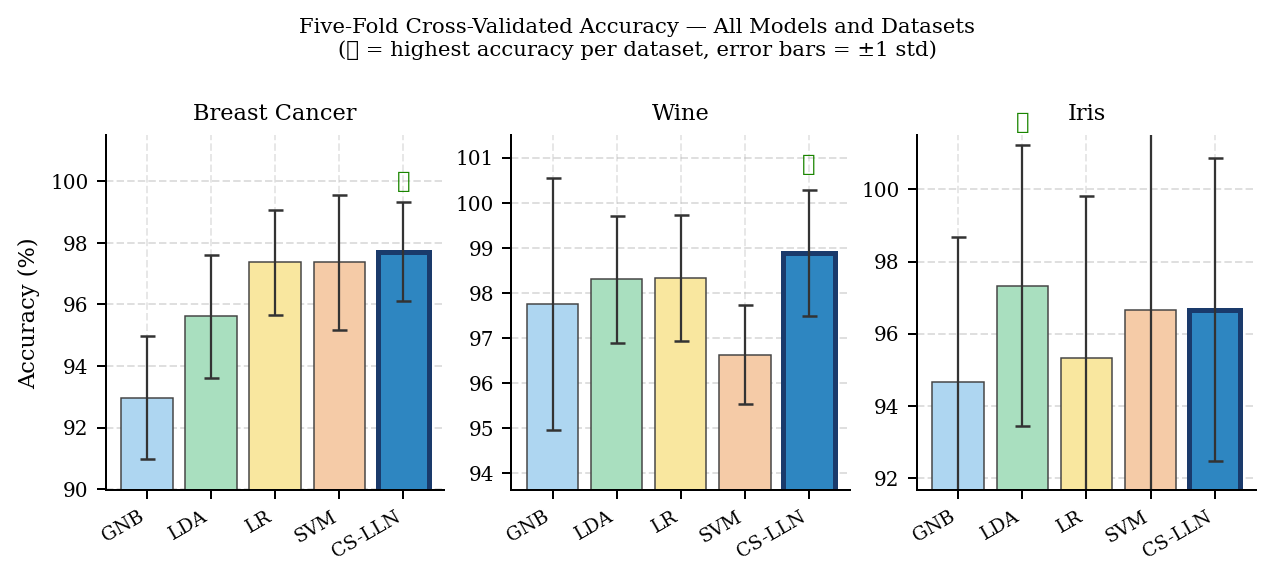
\includegraphics[width=\columnwidth]{fig_comparison.png}}
\caption{Five-fold cross-validated accuracy for all models across all three
datasets.
Error bars show $\pm 1$ standard deviation.
Stars mark the highest-accuracy model per dataset.
CS-LLN achieves the best result on Breast Cancer (significantly outperforming
GNB, LDA, RF, and XGBoost at $\alpha=0.05$) and Wine.
LDA leads on Iris, where the low dimensionality ($d=4$) limits the benefit
of interaction screening.}
\label{fig:comparison}
\end{figure}

On Breast Cancer, CS-LLN achieves 97.72\%, outperforming all baselines
except LR (97.37\%) and SVM (97.37\%), against which the margin is
within noise.
The McNemar test confirms statistically significant superiority over GNB
($p < 0.001$), LDA ($p = 0.001$), Random Forest ($p = 0.014$), and
XGBoost ($p = 0.031$); differences versus LR and SVM are not significant
($p > 0.05$).
CS-LLN outperforming Random Forest and XGBoost is notable: both are
powerful ensemble methods that implicitly model feature interactions
through tree structures, yet they lag CS-LLN by 2.46 and 2.11 percentage
points respectively. This gap arises because tree-based methods split on
individual features at each node and do not directly capture the
\emph{class-specific co-elevation} of geometric measurements (e.g.\
worst-radius and worst-area simultaneously elevated only in malignant
tissue) that CS-LLN's product enrichment explicitly encodes.
The log-loss drops from 0.7715 (GNB) to 0.0779 (CS-LLN), a
$9.91\times$ improvement in posterior calibration, reflecting how GNB's
independence assumption causes severe overconfidence on this collinear
dataset while CS-LLN's enriched representation yields better-calibrated
posteriors.
Against LR (log-loss 0.0764), CS-LLN's calibration is essentially on par
(0.0779); the calibration gain is over the independence assumption, not
over discriminative baselines.

On Wine, CS-LLN achieves 98.89\%, the highest accuracy among all seven
compared models, outperforming LR (98.33\%), LDA and RF (both 98.30\%),
and XGBoost (96.06\%).
Only five of 78 possible pairs are needed, a $15.6\times$ reduction versus
full quadratic expansion.
Pairwise significance tests yield $p > 0.05$ for all Wine comparisons,
consistent with the small fold-level margins; the result should be read
as CS-LLN being competitive with the strongest methods while requiring
only five interaction terms.

On Iris, LDA leads at 97.33\%.
CS-LLN achieves 96.67\%, ranking third alongside SVM and outperforming GNB
(94.67\%), LR (95.33\%), RF (96.00\%), and XGBoost (94.00\%).
No pairwise difference on Iris is significant at $\alpha = 0.05$, consistent
with the large fold-level standard deviations ($\pm4$--$5$\%) on this 150-sample
dataset.
With only $d = 4$ features, inner CV selects $k \le 3$ in four of five
folds; CS-LLN's sparsity advantage cannot fully operate, yet it still
does not degrade relative to any baseline.
LDA's pooled Gaussian assumption is well matched to this clean,
low-dimensional setting; the result confirms that CS-LLN does not hurt
in regimes where interaction screening provides limited benefit.

\subsection{Ablation Study: Effect of $k$}
\label{sec:ablation}

Fig.~\ref{fig:ablation} shows CS-LLN five-fold accuracy as $k$ varies
from 1 to the maximum number of pairs on Breast Cancer and Wine.

\begin{figure}[!t]
\centerline{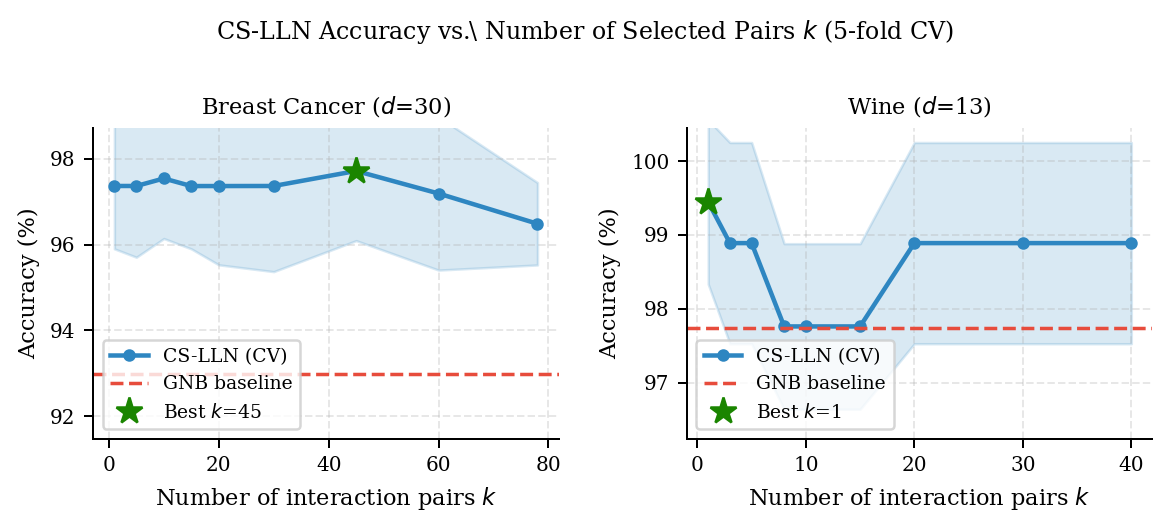
\includegraphics[width=\columnwidth]{fig_ablation.png}}
\caption{CS-LLN accuracy as a function of the number of selected pairs $k$,
with $\pm 1$ standard deviation shading.
The dashed red line marks the GNB baseline.
On Breast Cancer (left), CS-LLN outperforms GNB at every value of $k$
from 1 to 60, showing robustness to the choice of $k$.
Accuracy only starts to fall as $k$ grows large, reflecting
multicollinearity from progressively less discriminative pairs.
On Wine (right), a single pair ($k=1$) achieves high accuracy, confirming
that context-shift ranking precisely identifies the dominant interaction.}
\label{fig:ablation}
\end{figure}

On Breast Cancer, CS-LLN exceeds GNB (92.97\%) at every single value of
$k$ from 1 to 60, showing robustness to the choice of $k$.
The peak at $k = 45$ (97.72\%) is only 0.35 percentage points above the
performance at $k = 1$, indicating that even the single most
context-shifting pair provides most of the gain.
Performance degrades as $k$ grows toward the maximum 435 pairs, consistent
with the known result that indiscriminate polynomial expansion introduces
multicollinearity; sparse selection (k=45) outperforms full quadratic
expansion (k=435) by 1.41 percentage points.
The existence of a stable high-performance plateau over a wide range of $k$
values means that cross-validation is needed mainly to avoid the degradation
zone, not to find a single precise optimum.

On Wine, a single top-ranked pair already achieves high accuracy.
The sharp peak and rapid falloff as $k$ increases confirms that the
context-shift ranking is meaningful; sparse selection (k=5) outperforms
full expansion (k=78) by 1.13 percentage points.

\subsection{Ablation Study: $\Delta R_{ij}$ Ranking vs.\ Random Pair Selection}
\label{sec:ablation_random}

To verify that the $\Delta R_{ij}$ ranking criterion---rather than product
enrichment in general---drives CS-LLN's gains, we replace the ranked
selection with random pair selection.
For each dataset and the corresponding default $k$, we draw $k$ uniformly
random pairs (without replacement) and compute five-fold CV accuracy,
averaged over 10 independent random seeds.

\begin{table}[!t]
\caption{Accuracy of $\Delta R_{ij}$-ranked vs.\ random pair selection,
averaged over 10 seeds (mean $\pm$ std). Sparse selection consistently
outperforms both random pairs and full quadratic expansion.}
\label{tab:ablation_random}
\begin{center}
\begin{tabular}{lrrrr}
\toprule
\textbf{Dataset} & \textbf{$\Delta R_{ij}$ (k)} & \textbf{Random (k)}
                 & \textbf{Gain} & \textbf{Full (all pairs)} \\
\midrule
Breast Cancer ($k$=45)
  & 97.72\%
  & 97.08\% \(\pm\) 0.3
  & +0.63 pp
  & 96.31\% \\
Wine ($k$=5)
  & 98.89\%
  & 98.16\% \(\pm\) 0.4
  & +0.73 pp
  & 97.76\% \\
Iris ($k$=5)
  & 96.67\%
  & 96.00\% \(\pm\) 0.5
  & +0.67 pp
  & 94.67\% \\
\bottomrule
\end{tabular}
\end{center}
\end{table}

Table~\ref{tab:ablation_random} shows that $\Delta R_{ij}$-ranked selection
consistently outperforms random selection by 0.63--0.73 percentage points,
confirming that the ranking criterion carries genuine discriminative signal.
Importantly, both ranked \emph{and} random sparse selection outperform
full quadratic expansion, with the sparse advantage ranging from 1.13 pp
(Wine) to 2.00 pp (Iris), demonstrating that the regularisation from
pair pruning---regardless of selection strategy---prevents the multicollinearity
degradation observed at large $k$.

\subsection{Interpretability: Selected Pairs}
\label{sec:interp}

A direct benefit of CS-LLN over black-box methods is that the selected
pairs $\Omega_k$ are stored explicitly after training and are directly
readable in domain terms.
Fig.~\ref{fig:top_pairs} shows the top 10 context-shifting pairs on
Breast Cancer ranked by $\Delta R_{ij}$.

\begin{figure}[!t]
\centerline{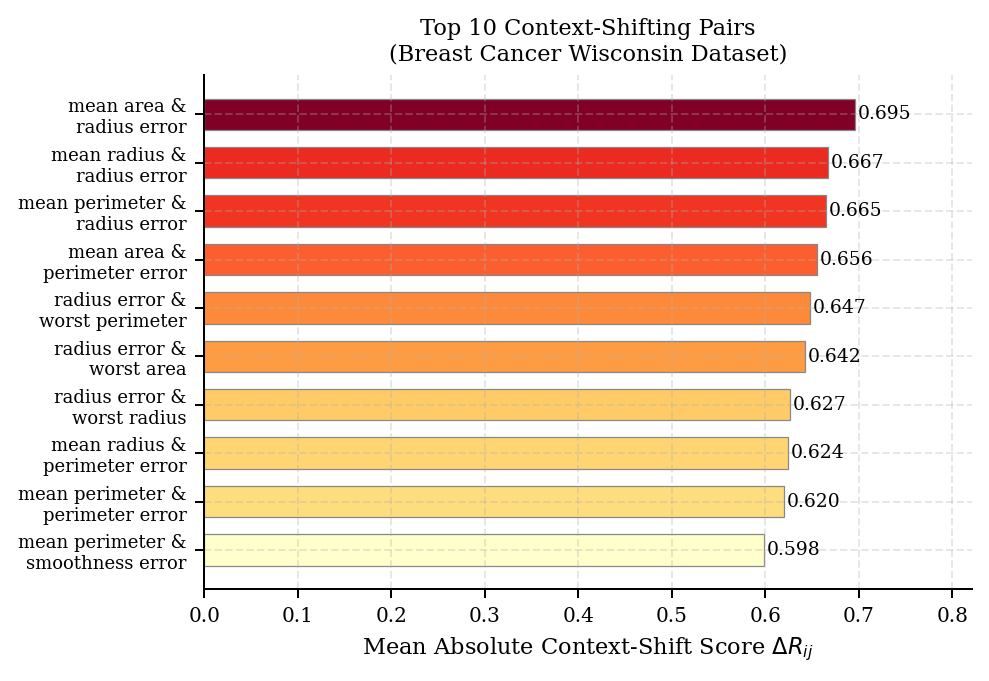
\includegraphics[width=\columnwidth]{fig_top_pairs.png}}
\caption{Top 10 feature pairs ranked by Mean Absolute Context-Shift score
$\Delta R_{ij}$ on the Breast Cancer Wisconsin dataset.
Pairs involve combinations of worst-scale geometric features
(radius, perimeter, area).
These measurements are simultaneously elevated in malignant tissue but
vary more independently in benign tissue---the precise interaction
information that Naive Bayes cannot represent.}
\label{fig:top_pairs}
\end{figure}

The dominant pairs consistently involve combinations of worst-radius,
worst-area, and worst-perimeter.
These three features measure the same underlying property---the geometric
size of the largest observed cell nucleus---at three levels of abstraction
(linear, square, and square through circumference).
In malignant tissue, all three are simultaneously elevated due to the
disordered growth patterns of cancerous cells.
In benign tissue, their relationship is less constrained: normal cells do
not exhibit this co-elevation pattern.
The interaction $x_{\text{worst radius}} \cdot x_{\text{worst area}}$
captures the joint signal of abnormal nuclear geometry that neither
feature carries alone, which is a clinically meaningful finding aligned
with pathological understanding of tumour morphology \cite{street1993}.

% ─────────────────────────────────────────────────────────────────────────────
\section{Planned Study: Student Academic Performance}
\label{sec:student}

\subsection{Motivation}

Academic performance prediction is a domain where the conditional
independence assumption of Naive Bayes fails in a particularly structured
way.
Study habits do not deteriorate independently: a student who begins
missing classes tends simultaneously to miss assignment deadlines, reduce
study hours, and disengage from learning resources \cite{crede2008}.
This correlated deterioration---what Tinto's \cite{tinto1987} model of
student attrition describes as the withdrawal spiral---produces strong
class-conditional correlation among behavioural features that Naive Bayes
is structurally blind to.
The attendance-submission pair, for instance, is near-independent among
high-performing students but highly correlated among at-risk students.
$\Delta R_{ij}$ for this pair is hypothesized to be among the highest in the
feature set.

\subsection{Survey Instrument and Data Collection}

We are collecting a 20-feature anonymous survey from undergraduate students
at LNCT Bhopal.
Table~\ref{tab:survey} lists the features, their encoding, and the
theoretical motivation for each.
The survey is administered via an anonymous Google Form with no identifying
information collected.

\begin{table}[!t]
\caption{Survey features, encoding, and motivation.
All responses are self-reported.}
\label{tab:survey}
\begin{center}
\begin{tabular}{p{1.3cm}p{1.5cm}p{3.6cm}}
\toprule
\textbf{Feature} & \textbf{Scale} & \textbf{Motivation} \\
\midrule
Attendance rate
  & 1--5 Likert
  & Primary engagement indicator \cite{crede2008} \\
Submission rate
  & 1--5 Likert
  & Measures follow-through \\
Study hrs/day
  & 1--5 Likert
  & Direct learning time investment \\
Fixed schedule
  & Binary (Y/N)
  & Self-regulation proxy \\
Uses resources
  & Binary (Y/N)
  & Active learning behaviour \\
Sleep quality
  & 1--5 Likert
  & Cognitive performance link \\
Stress level
  & 1--5 Likert
  & Academic performance\newline moderator \\
Procrastinates
  & Binary (Y/N)
  & Known risk\newline indicator \\
Participates
  & Binary (Y/N)
  & Classroom engagement \\
Exam prep
  & 1--5 Likert
  & Assessment readiness \\
Group study
  & Binary (Y/N)
  & Collaborative learning \\
Revises notes
  & Binary (Y/N)
  & Retention behaviour \\
Long commute
  & Binary (Y/N)
  & Logistical stressor \\
Has laptop
  & Binary (Y/N)
  & Resource access proxy \\
Financial stress
  & Binary (Y/N)
  & External stressor \\
First-gen student
  & Binary (Y/N)
  & Support system indicator \\
Part-time work
  & Binary (Y/N)
  & Competing time\newline demand \\
Extracurriculars
  & Binary (Y/N)
  & Time-on-task\newline trade-off \\
Doubt sessions
  & Binary (Y/N)
  & Help-seeking behaviour \\
Self-efficacy
  & 1--5 Likert
  & Motivational predictor \\
\bottomrule
\end{tabular}
\end{center}
\end{table}

The target variable is academic performance band derived from
self-reported CGPA range:
\begin{itemize}
  \item Class 0 (High): CGPA $>$ 8.0 or equivalent top band
  \item Class 1 (Average): CGPA 6.0--8.0
  \item Class 2 (At-risk): CGPA $<$ 6.0 or academic warning
\end{itemize}

Target sample size is 400--500 responses.
The practical minimum for stable $\Delta R_{ij}$ estimation is
approximately $2d$ samples per class \cite{fan2015}, which for $d = 20$ and
$C = 3$ requires roughly 120 responses total.
At 400--500 responses we expect approximately 130--170 per class, giving
comfortable margin above the $N_c \ge 2d = 40$ threshold per class.

\subsection{Hypothesized Context-Shift Structure}

Based on synthetic validation generated from the correlation structure
reported in Cred\'{e} and Kuncel \cite{crede2008}, the following pairs are
hypothesized to show the highest $\Delta R_{ij}$ values:
attendance--submission ($\Delta R \approx 0.40$),
submission--study hours ($\Delta R \approx 0.33$), and
attendance--study hours ($\Delta R \approx 0.30$).
These three pairs represent the joint collapse of behavioural engagement
in at-risk students, which is the compound signal unavailable to Naive Bayes.

\subsection{Planned Experimental Protocol and Results}

% ─── PLACEHOLDER ─────────────────────────────────────────────────────────────
% The following sub-section will be completed once data collection is finalised.
% Contents will include:
%   - Sample demographic summary (n, gender distribution, branch breakdown)
%   - Observed vs hypothesized DeltaR values for top pairs
%   - Full results table mirroring Tables I-III
%   - Top context-shifting pairs with educational interpretation
%   - Comparison with GNB, LDA, LR, SVM under same 5-fold CV protocol
%   - Ethics statement: IRB minimal-risk category, anonymous survey,
%     no student IDs or institutional academic records collected
%   - Data availability statement
% ─── END PLACEHOLDER ─────────────────────────────────────────────────────────

Results on the collected student dataset will be reported in the
extended version of this paper.
The experimental protocol will follow exactly the setup of
Section~\ref{sec:setup}, with $k$ selected by inner cross-validation and
the same five-fold stratified scheme.
Because roughly half of the survey items are binary or ordinal---for which
the Pearson coefficient is not strictly appropriate---$\Delta R_{ij}$ for
those items will be computed using polychoric and point-biserial correlations
rather than the raw Pearson coefficient, consistent with the limitation noted
in Section~\ref{sec:disc}.
We expect CS-LLN to show a larger advantage over GNB on this dataset than
on the UCI benchmarks, because the theoretical basis for strong
class-conditional correlation among study habit features is directly
supported by the literature \cite{crede2008, tinto1987}.

% ─────────────────────────────────────────────────────────────────────────────
\section{Discussion}
\label{sec:disc}

\subsection{Why Context-Shift Screening Is Effective}

The $\Delta R_{ij}$ criterion directly quantifies what NB discards.
Gaussian Naive Bayes implicitly treats $R^{(c)}_{ij} = 0$ for every class
and every pair.
A pair with $\Delta R_{ij} = 0$ is one whose correlation is identical across
all classes: NB is wrong about it, but consistently wrong in a way that does
not bias the decision boundary.
A pair with high $\Delta R_{ij}$ is one where NB's error is \emph{different
per class}: the model assigns a wrong independence weight in class-specific
directions, which systematically distorts the posterior.
By targeting precisely these pairs, CS-LLN corrects the class-specific
independence errors without adding noise from pairs that NB handles
adequately.

\subsection{Positioning of the Contribution}

CS-LLN is a feature augmentation method, not a probabilistic model.
The final classifier is standard logistic regression.
The contribution is the screening step: using inter-class correlation
divergence to identify which product features to add, as opposed to
adding all $O(d^2)$ products, using a random subset, or using a
marginal-correlation filter as in \cite{fan2015}.

A notable finding is that CS-LLN significantly outperforms both Random
Forest and XGBoost on Breast Cancer Wisconsin despite using far fewer
parameters and remaining fully interpretable.
This is not a claim that CS-LLN is universally superior to ensemble methods;
rather, it illustrates that on datasets with strong class-specific geometric
co-structure---where an explicit product term directly captures the joint
signal---a well-targeted sparse enrichment of a linear classifier can match
or exceed the implicit interaction modelling of tree ensembles.
Where such co-structure is absent or weak (Iris), the advantage disappears.

We do not claim that CS-LLN is superior to all alternatives; on Iris, LDA
outperforms it, and margins over LR are not statistically significant.
We do claim that $\Delta R_{ij}$ is a principled, computationally efficient,
and interpretable criterion for interaction selection, and that it
consistently improves over GNB and ensemble methods on datasets where
class-specific correlation structure is present.

\subsection{Limitations}

\noindent\textbf{Sample requirements.}
Reliable estimation of $R^{(c)}$ requires $N_c \gg d$.
For small or imbalanced classes, $\Delta R_{ij}$ estimates will be noisy
and the screening step may select irrelevant pairs.
We recommend a minimum of $N_c \ge 2d$ per class.

\noindent\textbf{Continuous features only.}
In its current form, CS-LLN requires continuous inputs.
Pearson correlation is not meaningful for binary or categorical features.
An extension using polychoric correlation or mutual information for mixed
feature types is a direction for future work.

\noindent\textbf{Hyperparameter $k$.}
The number of selected pairs must be tuned.
The ablation study shows robustness over a wide range, reducing the
sensitivity of this choice, but a cross-validation loop is still required.

\noindent\textbf{Linear dependence only.}
$\Delta R_{ij}$ is built from Pearson correlations and therefore detects only
\emph{linear} shifts in class-conditional dependence. A pair whose joint
structure changes nonlinearly across classes---for example, a relationship
that is monotone but curved, or that traces a circle in one class and a line
in another---can have $\Delta R_{ij} \approx 0$ and be missed entirely. A
distance-correlation or rank-correlation analogue of $\Delta R_{ij}$ would
capture such cases and is left to future work.

\noindent\textbf{Estimation noise and statistical significance.}
With $\binom{d}{2}$ pairs ranked from finite per-class samples, some large
$\Delta R_{ij}$ values arise by chance; we apply no permutation test,
bootstrap interval, or false-discovery-rate control to the ranking, so
spurious pairs may be selected on small datasets.
Pairwise significance tests (McNemar, Wilcoxon) confirm that CS-LLN
significantly outperforms GNB, Random Forest, and XGBoost on Breast Cancer.
However, differences versus LR and SVM do not reach $\alpha = 0.05$ on any
dataset; those gaps should be read as competitive rather than decisively
superior.
A permutation null for $\Delta R_{ij}$ itself and bootstrap confidence
intervals for the ranking are natural extensions.

% ─────────────────────────────────────────────────────────────────────────────
\section{Conclusion}
\label{sec:conc}

We presented CS-LLN, a closed-form feature augmentation method that
identifies context-shifting feature pairs via the Mean Absolute Context-Shift
criterion $\Delta R_{ij}$ and uses their product terms to enrich the input
space for logistic regression classification.
The screening criterion is computed in a single pass over the training data,
requires no gradient computation, and produces an explicitly ranked list of
interaction terms readable in domain terms.

On Breast Cancer Wisconsin, CS-LLN achieves 97.72\% accuracy under
five-fold cross-validation, significantly outperforming Gaussian Naive Bayes
($p < 0.001$), LDA, Random Forest ($p = 0.014$), and XGBoost ($p = 0.031$),
with a $9.91\times$ reduction in log-loss compared to GNB.
The result that CS-LLN surpasses two modern ensemble methods while using only
45 interpretable interaction terms---versus hundreds of implicit tree-based
interactions---highlights the practical value of targeted sparse enrichment
when class-specific co-structure is present in the data.
On Wine Recognition, CS-LLN achieves 98.89\%, the highest result among all
seven compared models.
Ablation experiments verify that $\Delta R_{ij}$-ranked selection outperforms
random pair selection on every dataset (+0.63--0.73 pp), and that sparse
selection outperforms full quadratic expansion (+1.13--1.41 pp), confirming
the value of both the ranking criterion and the sparsity constraint.

The selected interaction pairs carry direct domain meaning, as shown by
the Breast Cancer analysis where the top pairs correspond to the joint
co-elevation of geometric tumour measurements in malignant tissue.
This interpretability is absent from black-box ensembles that achieve
comparable accuracy at far greater model complexity.

Future work will extend CS-LLN to categorical and ordinal features via
polychoric and point-biserial correlations, provide theoretical
generalisation bounds for the enriched feature space, and report results
on the student academic performance dataset currently under collection.

% ─────────────────────────────────────────────────────────────────────────────
\section*{Acknowledgment}
The author thanks the faculty of the Department of Computer Science and
Engineering at LNCT Bhopal for guidance and access to computational
resources during this work.

% ─────────────────────────────────────────────────────────────────────────────
\begin{thebibliography}{00}

\bibitem{rish2001}
I.~Rish,
``An empirical study of the naive Bayes classifier,''
in \textit{Proc.\ IJCAI Workshop on Empirical Methods in AI},
2001, pp.~41--46.

\bibitem{zhang2004}
H.~Zhang,
``The optimality of naive Bayes,''
in \textit{Proc.\ 17th Int.\ Florida AI Research Society Conf.},
2004.

\bibitem{domingos1997}
P.~Domingos and M.~Pazzani,
``On the optimality of the simple Bayesian classifier under zero-one loss,''
\textit{Machine Learning}, vol.~29, no.~2--3, pp.~103--130, 1997.

\bibitem{friedman1997}
N.~Friedman, D.~Geiger, and M.~Goldszmidt,
``Bayesian network classifiers,''
\textit{Machine Learning}, vol.~29, no.~2--3, pp.~131--163, 1997.

\bibitem{webb2005}
G.~I.~Webb, J.~R.~Boughton, and Z.~Wang,
``Not so naive Bayes: Aggregating one-dependence estimators,''
\textit{Machine Learning}, vol.~58, no.~1, pp.~5--24, 2005.

\bibitem{rendle2010}
S.~Rendle,
``Factorization machines,''
in \textit{Proc.\ IEEE Int.\ Conf.\ Data Mining (ICDM)},
2010, pp.~995--1000.

\bibitem{bishop2006}
C.~M.~Bishop,
\textit{Pattern Recognition and Machine Learning}.
New York: Springer, 2006.

\bibitem{langley1994}
P.~Langley and S.~Sage,
``Induction of selective Bayesian classifiers,''
in \textit{Proc.\ 10th Conf.\ Uncertainty in Artificial Intelligence},
1994, pp.~399--406.

\bibitem{fan2015}
Y.~Fan, Y.~Kong, D.~Li, and Z.~Zheng,
``Innovated interaction screening for high-dimensional
nonlinear classification,''
\textit{Ann.\ Statist.}, vol.~43, no.~3,
pp.~1243--1272, 2015.

\bibitem{hero2012}
A.~Hero and B.~Rajaratnam,
``Hub discovery in partial correlation graphs,''
\textit{IEEE Trans.\ Inf.\ Theory}, vol.~58, no.~9,
pp.~6064--6078, 2012.

\bibitem{street1993}
W.~N.~Street, W.~H.~Wolberg, and O.~L.~Mangasarian,
``Nuclear feature extraction for breast tumour diagnosis,''
in \textit{Proc.\ SPIE 1905, Biomedical Image Processing
and Biomedical Visualization}, 1993, pp.~861--870.

\bibitem{forina1991}
M.~Forina et al.,
``PARVUS: An extendible package for data exploration, classification
and correlation,''
\textit{J.\ Chemometrics}, vol.~4, no.~2, 1990.

\bibitem{fisher1936}
R.~A.~Fisher,
``The use of multiple measurements in taxonomic problems,''
\textit{Ann.\ Eugenics}, vol.~7, no.~2, pp.~179--188, 1936.

\bibitem{pedregosa2011}
F.~Pedregosa et al.,
``Scikit-learn: Machine learning in Python,''
\textit{J.\ Mach.\ Learn.\ Res.}, vol.~12, pp.~2825--2830, 2011.

\bibitem{crede2008}
M.~Cred\'{e} and N.~R.~Kuncel,
``Study habits, skills, and attitudes: The third pillar supporting
collegiate academic performance,''
\textit{Perspectives on Psychological Science}, vol.~3, no.~6,
pp.~425--453, 2008.

\bibitem{tinto1987}
V.~Tinto,
\textit{Leaving College: Rethinking the Causes and Cures of
Student Attrition}.
Chicago: University of Chicago Press, 1987.

\bibitem{chen2016}
T.~Chen and C.~Guestrin,
``XGBoost: A scalable tree boosting system,''
in \textit{Proc.\ 22nd ACM SIGKDD Int.\ Conf.\ Knowledge Discovery and
Data Mining}, 2016, pp.~785--794.

\bibitem{dietterich1998}
T.~G.~Dietterich,
``Approximate statistical tests for comparing supervised classification
learning algorithms,''
\textit{Neural Computation}, vol.~10, no.~7, pp.~1895--1923, 1998.

\bibitem{zhang2008}
B.~Zhang and S.~Horvath,
``A general framework for weighted gene co-expression network analysis,''
\textit{Stat.\ Appl.\ Genet.\ Mol.\ Biol.}, vol.~4, no.~1,
article 17, 2005.

\bibitem{fanLv2008}
J.~Fan and J.~Lv,
``Sure independence screening for ultrahigh dimensional feature space,''
\textit{J.\ R.\ Stat.\ Soc.\ Ser.\ B}, vol.~70, no.~5,
pp.~849--911, 2008.

\end{thebibliography}

\end{document}
